% Hasznos doksik:
% https://tex.stackexchange.com/questions/42611/list-of-available-tikz-libraries-with-a-short-introduction
% https://www.overleaf.com/learn/latex/LaTeX_Graphics_using_TikZ:_A_Tutorial_for_Beginners_(Part_3)—Creating_Flowcharts

\documentclass[11pt]{beamer}
\usetheme{Szeged}
\usepackage[utf8]{inputenc}
\usepackage[magyar]{babel}
\usepackage[T1]{fontenc}
\usepackage{tikz}
\usepackage{graphicx}


\author{Tipográfiai rendszerek - \TeX}
\title{TikZ}
\date{2021.03.24.}

\newcommand{\tbs}{\textbackslash}


\begin{document}

\begin{frame}
\titlepage
\end{frame}


\begin{frame}{Mi az a TikZ?}
\begin{itemize}
\item Ehhez szükség van a \textbf{tikz} csomagra
\item A TikZ egy eszköz, amivel összetett grafikai elemeket hozhatunk létre \TeX{}-ben 
\item A TikZ-ben való munkához a \textbf{tikzpicture} környezetben kell dolgoznunk
	\begin{itemize}
	\item ha úsztatott ábrát szeretnénk, akkor ezt be kell ágyaznunk a \textbf{figure} környezetbe
	\end{itemize}
\item (x,y) koordináta rendszerben dolgozik
	\begin{itemize}
	\item A koordinátákat \textbf{vesszővel} a tizedesjegyeket \textbf{tizedes ponttal} választjuk el! Pl. (5.56,4.12)
	\end{itemize}
\item A TikZ ,,rétegekben'' dolgozik:
	\begin{itemize}
	\item a soronként lefelé haladva fedik le egymást az elemek
	\end{itemize}
\item a rajzok, vagy parancsok végét \textbf{pontosvessző} zárja!
\end{itemize}
\end{frame}

\begin{frame}{Nagyítás}
\begin{itemize}
\item Az alakzatokon lehet nagyítani, ezt pedig a \textbf{scale} paraméterrel tudjuk megadni
\item Lehet csak az egyik tengelyen is nagyítani, ebben az esetben az \textbf{xscale} vagy \textbf{yscale} paramétereket használjuk
\item De, lehet a két tengelyen külön nagyítást is használni, ebben az esetben e két paramétert egyszerre adjuk meg
	\begin{itemize}
	\item $\left[\right.$scale=x$\left.\right]$
	\end{itemize}
\end{itemize}

\end{frame}

\begin{frame}[fragile]{Néhány alakzat}
\begin{itemize}
\item Vonalat két, vagy több pont közé az alábbi paranccsal rajzolhatunk:
	\begin{itemize}
	\item \tbs draw (x1,y1)\verb|--|(x2,y2);
	\item \tbs draw (x1,y1)\verb|--|(x2,y2)\verb|--|(x3,y3);
	\end{itemize}
\item Kört az alábbi paranccsal rajzolhatunk:
	\begin{itemize}
	\item \tbs draw (x,y) circle (r);
	\item r=rádiusz azaz sugár
	\end{itemize}
\item Téglalapot az alábbi paranccsal rajzolhatunk:
	\begin{itemize}
	\item \tbs draw (x1,y1) rectangle (x2,y2);
	\item az első koordináta, ahol a toll elkezdi a rajzot, a második az azzal átlósan ellentétes pont
	\end{itemize}
\item Segédvonalak:
	\begin{itemize}
	\item \tbs draw [help lines] (x1,y1) grid (x2,y2);
	\item az első koordináta, ahol a toll elkezdi a rajzot, a második az azzal átlósan ellentétes pont
	\end{itemize}
\end{itemize}
\end{frame}

\begin{frame}{Vonalak opcionális paraméterei}
\begin{itemize}
\item A vonalakhoz is tartoznak opcionális paraméterek
\item Ezekből néhány:
	\begin{itemize}
	\item $\left[\right.$->$\left.\right]$
	\item $\left[\right.$<-$\left.\right]$
	\item $\left[\right.$<->$\left.\right]$
	\item $\left[\right.$|->$\left.\right]$
	\item $\left[\right.$<-|$\left.\right]$
	\end{itemize}
\end{itemize}
\end{frame}

\begin{frame}{Opcionális paraméterek - színek}
\begin{itemize}
\item Természetesen, az alakzatokat és a vonalakat lehet színezni is
\item Ehhez a parancs után az opcionális paraméterekhez kell megadni a színt angolul:
	\begin{itemize}
	\item white
	\item black
	\item red
	\item green
	\item blue
	\item cyan
	\item magenta
	\item yellow
	\end{itemize}
\item A színek telítettségét $\left[\right.$\textbf{szín!százalék}$\left.\right]$ módon adjuk meg. Pl. $\left[\right.$\textbf{red!20}$\left.\right]$
\end{itemize}
\end{frame}

\begin{frame}{Opcionális paraméterek - vonal típus és vastagság}
\begin{itemize}
\item A vonalak vastagsága is szabályozható:
	\begin{itemize}
	\item ultra thin
	\item very thin
	\item thin
	\item thick
	\item very thick
	\item ultra thick
	\end{itemize}
\item Illetve a $\left[\right.$\textbf{line width=x}$\left.\right]$ paraméterrel is
\item A vonalak típusát az alábbiakkal adhatjuk meg:
	\begin{itemize}
	\item dashed
	\item dotted
	\item \dots
	\end{itemize}
\end{itemize}
\end{frame}

\begin{frame}{Opcionális paraméterek - kitöltés}
\begin{itemize}
\item Az alakzatokat ki is tölthetjük színnel
\item Ebben az esetben a $\left[\right.$\textbf{fill=szín}$\left.\right]$ paramétert használjuk $\left[\right.$\textbf{fill=red!80}$\left.\right]$
\end{itemize}
\end{frame}

\begin{frame}{Függvények}
\begin{itemize}
\item Függvények kirajzolásához a \textbf{plot}-ot használhatjuk
	\begin{itemize}
	\item \tbs draw $\left[\right.$domain=szam$\left.\right]$ plot (\tbs valtozo, \{fuggveny\};
	\item \tbs draw $\left[\right.$domain=0:2*pi$\left.\right]$ plot (\tbs x, \{sin(\tbs x r)\});
	\end{itemize}
\item A domain a függvény megjeleníteni kívánt tartománya
\end{itemize}
\end{frame}

\begin{frame}{Megjegyzések}
\begin{itemize}
\item Az alakzat részeihez elhelyezhetünk megjegyzéseket
\item Erre a \textbf{\tbs node} parancs való
	\begin{itemize}
	\item \tbs node [hová] at (x,y) \{megjegyzés\};
	\end{itemize}
\item Használható elhelyezési paraméterek:
	\begin{itemize}
	\item above
	\item below
	\item left
	\item right
	\end{itemize}
\item Például:
	\begin{itemize}
	\item \tbs node [below] at (0,0) \{origó\};
	\end{itemize}
\end{itemize}
\end{frame}

\begin{frame}[fragile]{Ciklus}
\begin{itemize}
\item A TikZ-ben lehetőség van ciklussal is létrehozni alakzatokat
\item Erre a \textbf{\tbs foreach} parancs való
\item szintaxisa:
	\begin{itemize}
	\item \tbs foreach \tbs változó in \{skála\}
	\item a rajz maga;
	\end{itemize}
\item Például:
\end{itemize}

\begin{verbatim}
\foreach \x in {1,...,10}
	\foreach \y in {1,...,10}
       \draw[red, fill=blue, thick] 
       (\x,\y) rectangle (\x+0.5,\y+0.3);
\end{verbatim}
\end{frame}

\begin{frame}{Koordinátára hivatkozás 1.}
\begin{itemize}
\item A koordinátákat meg is címkézhetjük és később hivatkozhatunk rájuk
\item Egyik módszer a \tbs coordinate parancs
	\begin{itemize}
	\item \tbs coordinate (címke) at (x,y);
	\end{itemize}
\item például:
	\begin{itemize}
	\item \tbs coordinate (A) at (0,0);
	\end{itemize}
\end{itemize}
\end{frame}

\begin{frame}{Koordinátára hivatkozás 2.}
\begin{itemize}
\item A koordinátákat meg is címkézhetjük és később hivatkozhatunk rájuk
\item A másik módszer a \tbs path parancs - ezzel egyszerre fel is címkézhetjük
	\begin{itemize}
	\item \tbs path (x,y) coordinate(név) $\left[\right.$hová$\left.\right]$ node \{megjegyzés\};
	\end{itemize}
\item Például:
	\begin{itemize}
	\item \tbs path (0,0) coordinate(A) $\left[\right.$below$\left.\right]$ node \{A\};
	\end{itemize}
\end{itemize}
\end{frame}

\begin{frame}[fragile]{tikzstyle}
\begin{itemize}
\item Meghatározhatunk alap komponenseket, stílusokat is
\item \tbs tikzstyle\{név\} = [definíció]
\item \tbs tikzstyle \{név\}[változó] = [definíció1 \#1, definíció2 \#2]
\end{itemize}

\begin{verbatim}
\tikzstyle{alap}=[circle,draw=green];
\tikzstyle{mystyle}[green]=[draw=#1,fill=#2!20];
 
\node [alap] (v1) at (0,0) {szöveg};
\node [alap] (v2) at (5,0) {szöveg};

\draw (v1)--(v2);

\draw [mystyle] (10,10) rectangle (12,12);
\end{verbatim}
\end{frame}

\begin{frame}{Néhány minta}
\begin{tikzpicture}
\draw (0,1)--(0,5);
\draw (1,0)--(5,0);
\draw [->] (2,2)--(6,2);
\draw [<->] (3,3)--(6,3);
\draw [|->] (4,4)--(6,4);
\end{tikzpicture}
\end{frame}

\begin{frame}[fragile]
\begin{verbatim}
\begin{tikzpicture}
\draw (0,1)--(0,5);
\draw (1,0)--(5,0);
\draw [->] (2,2)--(6,2);
\draw [<->] (3,3)--(6,3);
\draw [|->] (4,4)--(6,4);
\end{tikzpicture}
\end{verbatim}
\end{frame}

\begin{frame}[fragile]
\begin{tikzpicture}
\draw [help lines] (0,0) grid (6,4);
\draw [<->] (0,4)--(0,0)--(6,0);
\path (0,0) node [below] {0};
\path (0,4) node [left] {Y};
\path (6,0) node [right] {X};
\end{tikzpicture}
\end{frame}

\begin{frame}[fragile]
\begin{verbatim}
\begin{tikzpicture}
\draw [help lines] (0,0) grid (6,4);
\draw [<->] (0,4)--(0,0)--(6,0);
\path (0,0) node [below] {0};
\path (0,4) node [left] {Y};
\path (6,0) node [right] {X};
\end{tikzpicture}
\end{verbatim}
\end{frame}


\begin{frame}
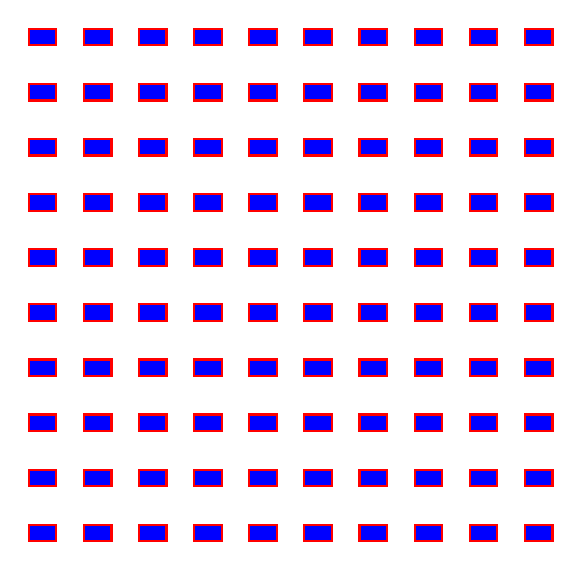
\begin{tikzpicture}[scale=0.7]
\foreach \x in {1,...,10}
	\foreach \y in {1,...,10}
       \draw[red, fill=blue, thick] (\x,\y) rectangle (\x+0.5,\y+0.3);
\end{tikzpicture}
\end{frame}

\begin{frame}[fragile]
\begin{verbatim}
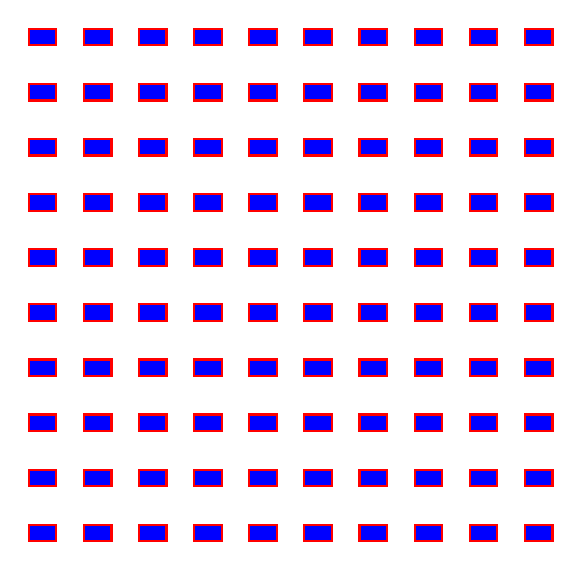
\begin{tikzpicture}[scale=0.7]
\foreach \x in {1,...,10}
	\foreach \y in {1,...,10}
       \draw[red, fill=blue, thick]
       (\x,\y) rectangle (\x+0.5,\y+0.3);
\end{tikzpicture}
\end{verbatim}
\end{frame}

\begin{frame}
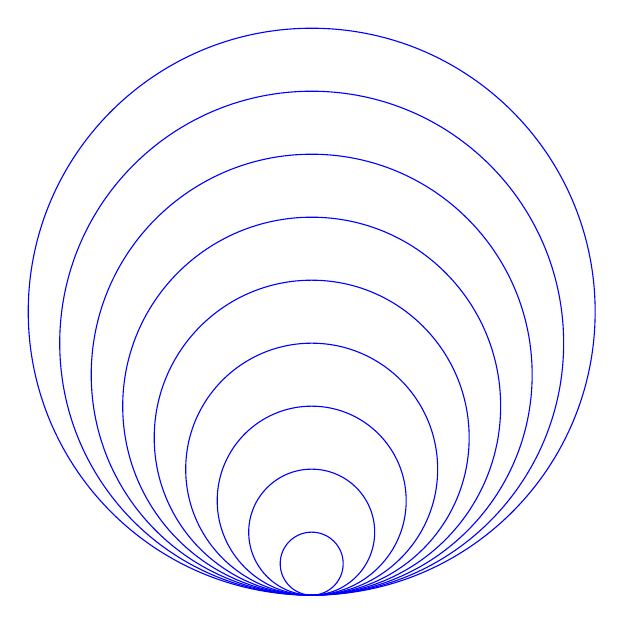
\begin{tikzpicture}[scale=0.4]

\foreach \x in {1,...,9}
       \draw[color=blue] (0,1*\x) circle (\x);

\end{tikzpicture}
\end{frame}

\begin{frame}[fragile]
\begin{verbatim}
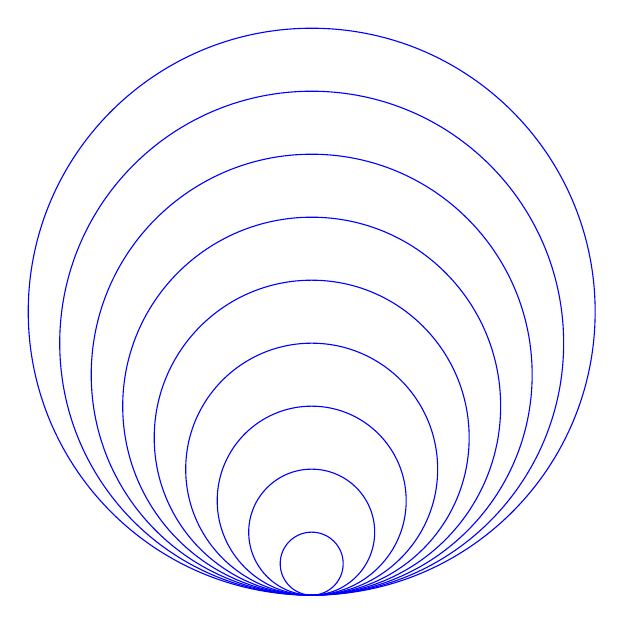
\begin{tikzpicture}[scale=0.4]

\foreach \x in {1,...,9}
       \draw[color=blue] (0,1*\x) circle (\x);

\end{tikzpicture}
\end{verbatim}
\end{frame}

\begin{frame}[fragile]
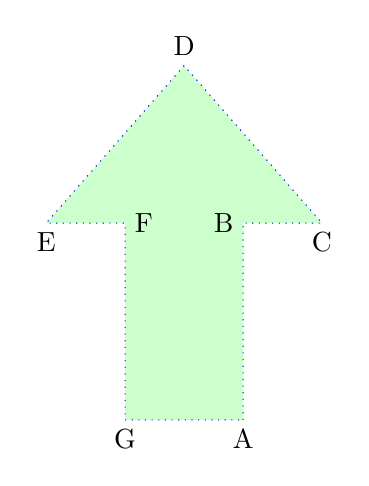
\begin{tikzpicture}[scale=0.5]
\coordinate (A) at (10,0);
\coordinate (B) at (10,5);
\coordinate (C) at (12,5);
\coordinate (D) at (8.5,9);
\coordinate (E) at (5,5);
\coordinate (F) at (7,5);
\coordinate (G) at (7,0);

\draw [dotted, blue, fill=green!20] (A)--(B)--(C)--(D)--(E)--(F)--(G)--(A);
\node [below] at (A) {A};
\node [left] at (B) {B};
\node [below] at (C) {C};
\node [above] at (D) {D};
\node [below] at (E) {E};
\node [right] at (F) {F};
\node [below] at (G) {G};
\end{tikzpicture}
\end{frame}

\begin{frame}[fragile]
\begin{verbatim}
\begin{tikzpicture}[scale=0.5]
\coordinate (A) at (10,0);
\coordinate (B) at (10,5);
\coordinate (C) at (12,5);
\coordinate (D) at (8.5,9);
\coordinate (E) at (5,5);
\coordinate (F) at (7,5);
\coordinate (G) at (7,0);
\end{verbatim}
\end{frame}


\begin{frame}[fragile]
\begin{verbatim}
\draw [dotted, blue, fill=green!20] (A)--(B)--(C)--
(D)--(E)--(F)--(G)--(A);
\node [below] at (A) {A};
\node [left] at (B) {B};
\node [below] at (C) {C};
\node [above] at (D) {D};
\node [below] at (E) {E};
\node [right] at (F) {F};
\node [below] at (G) {G};
\end{tikzpicture}
\end{verbatim}
\end{frame}


\end{document}